\documentclass[12pt,a4paper]{report}
\usepackage[margin=2.5cm]{geometry}
\usepackage{amsmath}
\usepackage{graphicx}
\usepackage{caption}
\usepackage{subcaption}
\usepackage[nottoc,numbib]{tocbibind}
\linespread{1.3}

\begin{document}

\begin{titlepage}
	\begin{center}
		\large
		\vspace*{1cm}
        		
 		\textbf{On Hitting a Moving Target}
        
		\vspace{0.5cm}
		By
        
		\vspace{1.5cm}
        
		\textbf{Romilly Djee Yin Hills}\\

		\vspace{1.5cm}

		\today \\
		\copyright Romilly Djee Yin Hills\\
        
	\end{center}
\end{titlepage}

%%%%%%%%%%

\chapter{Introduction}
\label{Introduction}

Notes on hitting a moving target in three dimensions.

\section{The Problem}
\label{section_the_problem}

I encountered this problem while investigaing the creation of a video game using the Unity game engine\cite{unity_webpage}. The game is to be set in space and (in the early stages of development) I required a space ship to be able to shoot an asteroid (to be refered to as the 'target') with a slow projectile.

If the target is stationary we have no issues hitting the target, the 'gun' can simply be aimed at the target, and, after some time (for this scale I wanted the projectile to have to travel for more than one second) the projectile would hit the target. However, if the target is moving (with a constant velocity) by the time the projectile reaches the location of the target, the target has changed position and the projectile misses.


\section{The Solution}
\label{section_the_solution}

To overcome this problem, instead of aiming directly at the target, we must calculate where the target will be after some time and aim at that location instead. In this case 'some time' is the time our projectile will take to travel to that same location which is depicted in Figure \ref{Moving_target_diagram_flat.png}.

\begin{figure}
	\centerline{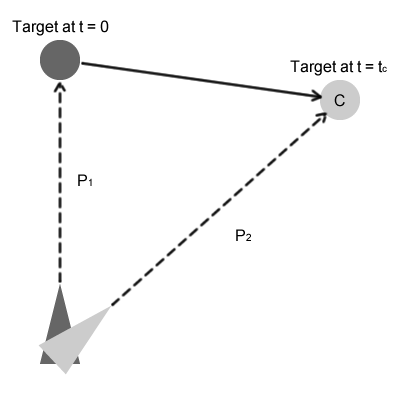
\includegraphics[scale=0.8]{Moving_target_diagram_flat.png}}
	\caption{A diagram depicting the paths of two projectiles $P_{1}$ and $P_{2}$, a moving target at $t=0$ and $t=t_{c}$ (with $t_{c} > t$), and the point $C$ where the target and $P_{2}$ will collide.}
	\label{Moving_target_diagram_flat.png}
\end{figure}

%%%%%%%%%%

\chapter{Calculating the Collision Location for Objects with Constant Velocities}
\label{Calculating Collision Locations for Constant Velocities}

We must first introduce a few definitions; we have a target $T_{i}$ at the point $\vec{T} = \left[T_{x}, T_{y}, T_{z}\right]$ with the velocity $\vec{V} = \left[V_{x},V_{y},V_{z}\right]$ and a projectile $P_{i}$ at the point $\vec{P} = \left[P_{x}, P_{y}, P_{z}\right]$ with a speed $s$. We wish to calculate the location $\vec{C}$ that $P_{i}$ and $T_{i}$ will collide.

The distance $d$ between $\vec{P}$ and $\vec{C}$ can be calulated with the Pythagoras Theorem

\begin{equation}
	d^{2} = \left(C_{x}-P_{x}\right)^{2} + \left(C_{y}-P_{y}\right)^{2} + \left(C_{z}-P_{z}\right)^{2}
	\label{d_pythagoras}
\end{equation}
and 
\begin{equation}
	d = st
	\label{d_st}
\end{equation}
where $t$ is the amount of time until the collision will occur. From the equations of linear motion for the target, we also know that
\begin{align}
	C_{x} = T_{x} + V_{x}t
	\hspace{1cm}
	C_{y} = T_{y} + V_{y}t
	\hspace{1cm}
	C_{z} = T_{z} + V_{z}t.
	\label{cxyz}
\end{align}
We can then substitute equation (\ref{d_st}) into the left hand side of equation (\ref{d_pythagoras}) and the definitions of $C_{x,y,z}$ from equation (\ref{cxyz}) into the right hand side of equation (\ref{d_pythagoras}) to produce the quadratic equation
\begin{equation}
	s^{2}t^{t} = \left(T_{x} + V_{x}t - P_{x}\right)^{2} + \left(T_{y} + V_{y}t - P_{y}\right)^{2} + \left(T_{z} + V_{z}t - P_{z}\right)^{2}
	\label{s2t2}
\end{equation}
with $t$ as the unknown. Equation (\ref{s2t2}) can be expanded and rearraged to the general form of the quadratic equation
\begin{align}
	0 =&\left(V_{x}^{2}+V_{y}^{2}+V_{z}^{2} - s^2\right)t^{2}\\
 	&+ 2\left(V_{x}\left(T_{x}- P_{x}\right) + V_{y}\left(T_{y}- P_{y}\right)+V_{z}\left(T_{z}- P_{z}\right)\right)t\\
	&+ T_{x}^{2} + T_{y}^{2} + T_{z}^{2} + P_{x}^{2} + P_{y}^{2} + P_{z}^{2}\\
	&- 2\left(T_{x}P_{x} + T_{y}P_{y} + T_{z}P_{z}\right).
\end{align}
The general quadratic equation $ax^{2}+bx+c$ has two solutions given by
\begin{equation}
	x = \frac{-b \pm \sqrt{b^{2}-4ac}}{2a},
	\label{quadratic_formula}
\end{equation}
therefore with the definitions
\begin{align}
	x &= t\\
	a &= V_{x}^{2}+V_{y}^{2}+V_{z}^{2} - s^2\\
	b &= 2\left(V_{x}\left(T_{x}- P_{x}\right) + V_{y}\left(T_{y}- P_{y}\right)+V_{z}\left(T_{z}- P_{z}\right)\right)\\
	c &= T_{x}^{2} + T_{y}^{2} + T_{z}^{2} + P_{x}^{2} + P_{y}^{2} + P_{z}^{2} - 2\left(T_{x}P_{x} + T_{y}P_{y} + T_{z}P_{z}\right)
\end{align}
we can calculate $t$ from equation (\ref{quadratic_formula}).

Now that we have the amount of time until the collision will occur $t$, the location of the collision $\vec{C}$ can simply be calculated by  
\begin{equation}
	\vec{C} = \vec{T}+\vec{V}t
\end{equation}



\begin{thebibliography}{10}
%% https://gamedevelopment.tutsplus.com/tutorials/unity-solution-for-hitting-moving-targets--cms-29633

\bibitem{unity_webpage} https://unity.com/

\end{thebibliography}

\end{document}